\let\negmedspace\undefined
\let\negthickspace\undefined
%\RequirePackage{amsmath}
\documentclass[journal,12pt,twocolumn]{IEEEtran}
%
% \usepackage{setspace}
\usepackage{gensymb}
%\doublespacing
%\singlespacing
%\usepackage{silence}
%Disable all warnings issued by latex starting with "You have..."
%\usepackage{graphicx}
\usepackage{amssymb}
%\usepackage{relsize}
\usepackage{amsmath}
%\usepackage{amsthm}
%\interdisplaylinepenalty=2500
%\savesymbol{iint}
%\usepackage{txfonts}
%\restoresymbol{TXF}{iint}
%\usepackage{wasysym}
\usepackage{amsthm}
%\usepackage{pifont}
%\usepackage{iithtlc}
% \usepackage{mathrsfs}
% \usepackage{txfonts}
\usepackage{stfloats}
% \usepackage{steinmetz}
\usepackage{bm}
% \usepackage{cite}
% \usepackage{cases}
% \usepackage{subfig}
%\usepackage{xtab}
\usepackage{longtable}
%\usepackage{multirow}
%\usepackage{algorithm}
%\usepackage{algpseudocode}
\usepackage{enumitem}
\usepackage{mathtools}
\usepackage{tikz}
% \usepackage{circuitikz}
% \usepackage{verbatim}
%\usepackage{tfrupee}
\usepackage[breaklinks=true]{hyperref}
%\usepackage{stmaryrd}
%\usepackage{tkz-euclide} % loads  TikZ and tkz-base
%\usetkzobj{all}
\usepackage{listings}
\usepackage{color}                                            %%
\usepackage{array}                                            %%
\usepackage{longtable}                                        %%
\usepackage{calc}                                             %%
\usepackage{multirow}                                         %%
\usepackage{hhline}                                           %%
\usepackage{ifthen}                                           %%
%optionally (for landscape tables embedded in another document): %%
\usepackage{lscape}     
% \usepackage{multicol}
% \usepackage{chngcntr}
%\usepackage{enumerate}

%\usepackage{wasysym}
%\newcounter{MYtempeqncnt}
\DeclareMathOperator*{\Res}{Res}
\DeclareMathOperator*{\equals}{=}
%\renewcommand{\baselinestretch}{2}
\renewcommand\thesection{\arabic{section}}
\renewcommand\thesubsection{\thesection.\arabic{subsection}}
\renewcommand\thesubsubsection{\thesubsection.\arabic{subsubsection}}

\renewcommand\thesectiondis{\arabic{section}}
\renewcommand\thesubsectiondis{\thesectiondis.\arabic{subsection}}
\renewcommand\thesubsubsectiondis{\thesubsectiondis.\arabic{subsubsection}}

% correct bad hyphenation here
\hyphenation{op-tical net-works semi-conduc-tor}
\def\inputGnumericTable{}                                 %%

\lstset{
	%language=C,
	frame=single, 
	breaklines=true,
	columns=fullflexible
}
%\lstset{
	%language=tex,
	%frame=single, 
	%breaklines=true
	%}
\begin{document}
	
	%
	
	
	\newtheorem{theorem}{Theorem}[section]
	\newtheorem{problem}{Problem}
	\newtheorem{proposition}{Proposition}[section]
	\newtheorem{lemma}{Lemma}[section]
	\newtheorem{corollary}[theorem]{Corollary}
	\newtheorem{example}{Example}[section]
	\newtheorem{definition}[problem]{Definition}
	%\newtheorem{thm}{Theorem}[section] 
	%\newtheorem{defn}[thm]{Definition}
	%\newtheorem{algorithm}{Algorithm}[section]
	%\newtheorem{cor}{Corollary}
	\newcommand{\BEQA}{\begin{eqnarray}}
		\newcommand{\EEQA}{\end{eqnarray}}
	\newcommand{\define}{\stackrel{\triangle}{=}}
	\newcommand*\circled[1]{\tikz[baseline=(char.base)]{
			\node[shape=circle,draw,inner sep=2pt] (char) {#1};}}
	\bibliographystyle{IEEEtran}
	%\bibliographystyle{ieeetr}
	
	
	\providecommand{\mbf}{\mathbf}
	\providecommand{\pr}[1]{\ensuremath{\Pr\left(#1\right)}}
	\providecommand{\qfunc}[1]{\ensuremath{Q\left(#1\right)}}
	\providecommand{\sbrak}[1]{\ensuremath{{}\left[#1\right]}}
	\providecommand{\lsbrak}[1]{\ensuremath{{}\left[#1\right.}}
	\providecommand{\rsbrak}[1]{\ensuremath{{}\left.#1\right]}}
	\providecommand{\brak}[1]{\ensuremath{\left(#1\right)}}
	\providecommand{\lbrak}[1]{\ensuremath{\left(#1\right.}}
	\providecommand{\rbrak}[1]{\ensuremath{\left.#1\right)}}
	\providecommand{\cbrak}[1]{\ensuremath{\left\{#1\right\}}}
	\providecommand{\lcbrak}[1]{\ensuremath{\left\{#1\right.}}
	\providecommand{\rcbrak}[1]{\ensuremath{\left.#1\right\}}}
	\theoremstyle{remark}
	\newtheorem{rem}{Remark}
	\newcommand{\sgn}{\mathop{\mathrm{sgn}}}
	\providecommand{\abs}[1]{\left\vert#1\right\vert}
	\providecommand{\res}[1]{\Res\displaylimits_{#1}} 
	\providecommand{\norm}[1]{\left\lVert#1\right\rVert}
	%\providecommand{\norm}[1]{\lVert#1\rVert}
	\providecommand{\mtx}[1]{\mathbf{#1}}
	\providecommand{\mean}[1]{E\left[ #1 \right]}
	\providecommand{\fourier}{\overset{\mathcal{F}}{ \rightleftharpoons}}
	%\providecommand{\hilbert}{\overset{\mathcal{H}}{ \rightleftharpoons}}
	\providecommand{\system}{\overset{\mathcal{H}}{ \longleftrightarrow}}
	%\newcommand{\solution}[2]{\textbf{Solution:}{#1}}
	\newcommand{\solution}{\noindent \textbf{Solution: }}
	\newcommand{\cosec}{\,\text{cosec}\,}
	\providecommand{\dec}[2]{\ensuremath{\overset{#1}{\underset{#2}{\gtrless}}}}
	\newcommand{\myvec}[1]{\ensuremath{\begin{pmatrix}#1\end{pmatrix}}}
	\newcommand{\mydet}[1]{\ensuremath{\begin{vmatrix}#1\end{vmatrix}}}
	%\numberwithin{equation}{section}
	%\numberwithin{problem}{section}
	%\numberwithin{definition}{section}
	\makeatletter
	\@addtoreset{figure}{problem}
	\makeatother
	
	\let\StandardTheFigure\thefigure
	\let\vec\mathbf
	%\renewcommand{\thefigure}{\theproblem.\arabic{figure}}
	
	%\setlist[enumerate,1]{before=\renewcommand\theequation{\theenumi.\arabic{equation}}
		%\counterwithin{equation}{enumi}
		
		
		%\renewcommand{\theequation}{\arabic{subsection}.\arabic{equation}}
		\def\putbox#1#2#3{\makebox[0in][l]{\makebox[#1][l]{}\raisebox{\baselineskip}[0in][0in]{\raisebox{#2}[0in][0in]{#3}}}}
		\def\rightbox#1{\makebox[0in][r]{#1}}
		\def\centbox#1{\makebox[0in]{#1}}
		\def\topbox#1{\raisebox{-\baselineskip}[0in][0in]{#1}}
		\def\midbox#1{\raisebox{-0.5\baselineskip}[0in][0in]{#1}}
	
		
		\title{
			AI1110 : Probability And Random Variables
                                     Assignment 2 
                        
		}
		\author{ 
		            Kota Vignan(CS21BTECH11029)
		}	
		%\title{
			%	\logo{Matrix Analysis through Octave}{\begin{center}\includegraphics[scale=.24]{tlc}\end{center}}{}{HAMDSP}
			%}
		
		
		% paper title
		% can use linebreaks \\ within to get better formatting as desired
		%\title{Matrix Analysis through Octave}
		%
		%
		% author names and IEEE memberships
		% note positions of commas and nonbreaking spaces ( ~ ) LaTeX will not break
		% a structure at a ~ so this keeps an author's name from being broken across
		% two lines.
		% use \thanks{} to gain access to the first footnote area
		% a separate \thanks must be used for each paragraph as LaTeX2e's \thanks
		% was not built to handle multiple paragraphs
		%
		
		%\author{<-this % stops a space
			%\thanks{}}
		%}
	% note the % following the last \IEEEmembership and also \thanks - 
	% these prevent an unwanted space from occurring between the last author name
	% and the end of the author line. i.e., if you had this:
	% 
	% \author{....lastname \thanks{...} \thanks{...} }
	%                     ^------------^------------^----Do not want these spaces!
	%
	% a space would be appended to the last name and could cause every name on that
	% line to be shifted left slightly. This is one of those "LaTeX things". For
	% instance, "\textbf{A} \textbf{B}" will typeset as "A B" not "AB". To get
	% "AB" then you have to do: "\textbf{A}\textbf{B}"
	% \thanks is no different in this regard, so shield the last } of each \thanks
% that ends a line with a % and do not let a space in before the next \thanks.
% Spaces after \IEEEmembership other than the last one are OK (and needed) as
% you are supposed to have spaces between the names. For what it is worth,
% this is a minor point as most people would not even notice if the said evil
% space somehow managed to creep in.
%\WarningFilter{latex}{LaTeX Warning: You have requested, on input line 117, version}
% The paper headers
%\markboth{Journal of \LaTeX\ Class Files,~Vol.~6, No.~1, January~2007}%
%{Shell \MakeLowercase{\textit{et al.}}: Bare Demo of IEEEtran.cls for Journals}
% The only time the second header will appear is for the odd numbered pages
% after the title page when using the twoside option.
% 
% * Note that you probably will NOT want to include the author's *
% * name in the headers of peer review papers.                   *
% You can use \ifCLASSOPTIONpeerreview for conditional compilation here if
% you desire.
% If you want to put a publisher's ID mark on the page you can do it like
% this:
%\IEEEpubid{0000--0000/00\$00.00~\copyright~2007 IEEE}
% Remember, if you use this you must call \IEEEpubidadjcol in the second
% column for its text to clear the IEEEpubid mark.
% make the title area
\maketitle
\newpage
\bigskip
\begin{abstract}
   This document provides solution of Assignment 2(ICSE 2018 12 Q.5(a))
\end{abstract}
 \textbf{ Question 5(a):}
   Show that the function $ f\brak{x} = \begin{cases}
                                         x^2, & x \leq 1 \\ 
                                        \frac{1}{x}, & x > 1
                                        \end{cases}$is continuous at $ x = 1 $ but not differentiable.\\
 \textbf{ Key Concept : }
  \begin{enumerate}
      \item  A function f is said to be continuous at $x = a$,iff the following three conditions satisfied. 
            \begin{enumerate}[label=\roman*]
                \item The limit $\lim_{x \to a}f\brak{x}$ should exist and it is finite.
                \item The functional value $f\brak{a}$ should exist and it is finite.
                \item $\lim_{x \to a}f\brak{x}$ = $f\brak{a}$.
            \end{enumerate}
      \item  A function f is said to be differentiable at $x=a$ if and only if the limit,
           \[
               lim_{h \to 0}\frac{f\brak{a + h} - f\brak{a}}{h}
           \]  exists.
                 
  \end{enumerate}
 \textbf{ Solution :}
  Given  
            \begin{equation*} 
                 f\brak{x}  = \begin{cases}
                              x^2,  & x \leq 1 \\
                              \frac{1}{x} , & x  >  1
                           \end{cases}
            \end{equation*}  
   We can say f is continuous at $x = 1$,iff 
            \begin{align}
                 \lim_{x \to 1}f\brak{x} &= f\brak{1}
            \end{align}
    In other words f should satisfy,
            \begin{align}
                 f\brak{1^-} =f\brak{1^+} =f\brak{1} 
            \end{align}
    where,
            \begin{align}
                 f\brak{1^-} &=  \lim_{h\to0}f\brak{1-h}\\
                 f\brak{1^+} &=  \lim_{h\to0}f\brak{1+h}
            \end{align}
            \begin{align}
                 f\brak{1} &= 1\label{eq 5}
            \end{align}
    Now,
            \begin{align}
                 f\brak{1^-}  &= \lim_{h\to0}f\brak{1-h}\\
                                    &= \lim_{h\to0}  \brak{1-h}^2\\
                 \implies f\brak{1^-} &= 1\label{eq 8}
            \end{align}
    And,
            \begin{align}
                 f\brak{1^+} &= \lim_{h\to0}f\brak{1+h}\\
                                    &= \lim_{h\to0} \frac{1}{\brak{1+h}}\\
                 \implies f\brak{1^+} &= 1\label{eq 11}
            \end{align}
    Using \eqref{eq 5} ,\eqref{eq 8},\eqref{eq 11},we can say that f is continuous at $ x = 1 $ and this can be seen in Fig $\ref{fig:Figure 1}$.\\
    Now from the concept of differentiability,we can say f is differentiable at $ x = 1 $ iff the limit,
             \[
                lim_{h \to 0}\frac{f\brak{1 + h} - f\brak{1}}{h}
             \] exists.\\
    In that case f should satisfy,
            \begin{align}
                 \lim_{h \to 0}\frac{f\brak{1 + h} - f\brak{1}}{h}  &=  lim_{h \to 0}\frac{f\brak{1} - f\brak{1-h}}{h}\label{eq 12} % LHD = RHD
            \end{align}
 \textbf{LHS:}
            \begin{align}
                 \lim_{h \to 0}\frac{f\brak{1 + h} - f\brak{1}}{h} & = \lim_{h \to 0}\frac{\brak{\frac{1}{\brak{1+h}}} - 1}{h}\\
                 & = \lim_{h \to 0}\frac{{\brak{1 - \brak{1 + h}}}}{h\brak{1 + h}}\\
                 & = \lim_{h \to 0}\frac{-h}{h\brak{1 + h}}\\                                       
                 & = \lim_{h \to 0}\frac{-1}{\brak{1 + h}}\\                         
                 & = -1\\
                 \implies \lim_{h \to 0}\frac{f\brak{1 + h} - f\brak{1}}{h} & = -1.
            \end{align}       
 \textbf{RHS:}
            \begin{align}
                 \lim_{h \to 0}\frac{f\brak{1} - f\brak{1-h}}{h}  &= \lim_{h \to 0}\frac{1 -\brak{  \brak{1 -h}^2}}{h}\\
                                                                                      &= \lim_{h \to 0}\frac{-\brak{2h - h^2}}{h}\\
                    &= \lim_{h \to 0}\frac{h\brak{2 - h}}{h}\\                                       
                &= \lim_{h \to 0}-\brak{2 - h}\\    & = 2\\
                 \implies  \lim_{h \to 0}\frac{f\brak{1} - f\brak{1-h}}{h} &= 2.\\
                 \therefore LHS &\neq RHS \nonumber
            \end{align}
    Hence, function $f(x)$ is not differentiable at $ x = 1 $.This can be seen in Fig $\ref{fig:Figure 2}$.\\
    Therefore, we proved that  $ f\brak{x} = \begin{cases}
                                         x^2, & x \leq 1 \\ 
                                        \frac{1}{x}, & x > 1
                                        \end{cases} $ is continuous at $ x = 1 $ but not differentiable. 
\begin{figure}[h!]
     \centering
     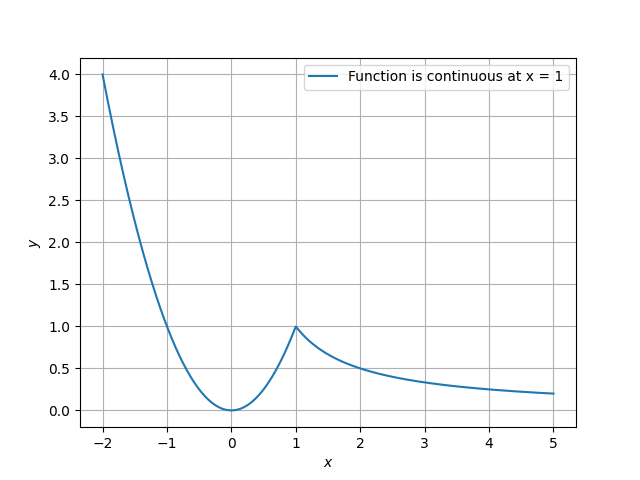
\includegraphics[width=\columnwidth]{Figs/Figure_1.png}
     \caption{}
     \label{fig:Figure 1}
\end{figure}
\begin{figure}[h!]
     \centering
     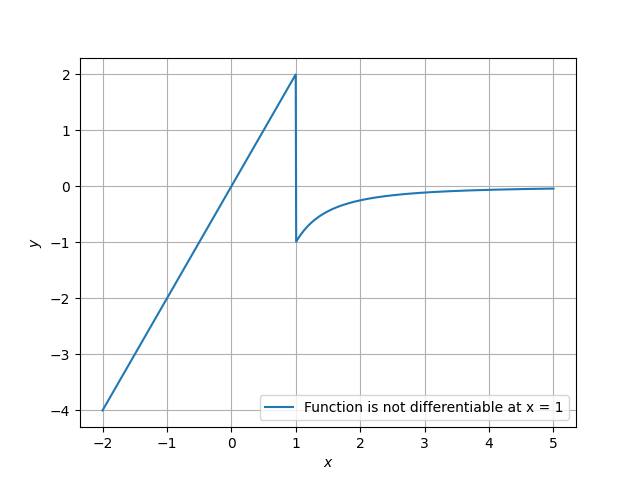
\includegraphics[width=\columnwidth]{Figs/Figure_2.png}
     \caption{}
     \label{fig:Figure 2}
\end{figure}
\end{document}